\documentclass{book}
\usepackage[latin1]{inputenc}    
\usepackage[T1]{fontenc}
\usepackage[german]{babel}     
\usepackage{graphicx}
\pagestyle{headings}
\usepackage[top=2cm, bottom=3cm, left=2cm, right=2cm]{geometry}
\usepackage{wrapfig}
\usepackage{hyperref}
\usepackage{float}

\hypersetup{
backref=true, %permet d'ajouter des liens dans...
pagebackref=true,%...les bibliographies
hyperindex=true, %ajoute des liens dans les index.
colorlinks=true, %colorise les liens
breaklinks=true, %permet le retour � la ligne dans les liens trop longs
urlcolor= black, %couleur des hyperliens
linkcolor= black, %couleur des liens internes
bookmarks=true, %cr�� des signets pour Acrobat
bookmarksopen=true, %si les signets Acrobat sont cr��s,
%les afficher compl�tement.
pdftitle={Designing eines Computerspiels}, %informations apparaissant dans
pdfauthor={Samuel Gauthier}, %dans les informations du document
pdfsubject={Windows XP} %sous Acrobat.
}

\begin{document}
\begin{titlepage}
\centering


\includegraphics[width=.75\textwidth]{logo.png}

\Huge{Designing eines Computerspiels\\ \vspace{300pt}}
\Large{Samuel Gauthier\\Maturarbeit 2012\\}
\small{\textit{Betreuer:} Thomas Vogelsanger\\}
\end{titlepage}
\tableofcontents
\frontmatter
\chapter{Vorwort}
Als ich 4 war bekam ich meinen ersten eigenen Computer: ein Maxdata 286 mit 12Mhz Prozessor 20MB Festplatte 1MB Ram. Auf dessen lief noch DOS. Von dieser Zeit an, begann ich die IT Welt zu entdecken. Mein erstes Spiele war das Golf Spiel PGA Tour 96. Ich verbrachte Stunden um zu verstehen wie man am besten Golf spielen konnte. Ein anderes Spiel war ein Spiel das zu zweit gespielt wurde und indem das Ziel den gegnerischen Affen mit Bananen zu beschiessen war; Wind und Gravitation kamen auch in Frage. Als ich manchmal genug von spielen hatte probierte ich alle m�glichen Einstellungen des Computers aus. Nat�rlich von Zeit st�rzte meinen Computer ab und mein Vater musste ihn wieder herrichten. Einige Jahre sp�ter bekam ich meinen zweiten Computer: ein --- mit mit ---Mhz Prozessor ---MB Festplatte ---MB Ram. (Schon hier sieht man die rasante Entwicklung der Informatik die in den n�chsten Jahren noch gr�sser geworden ist.) Danach spielte ich mit dem Valdo Spiel. Ein "Adventure Thinking" Game. Auch hier brachte ich viele Zeit damit. Z.B. als der Lothard Sturm die ganze Schweiz durchsch�ttelte spielten meinen Bruder, meinen Vater und ich mit diesem Spiel. Doch weil es von Zeit zu Zeit Stromst�rungen gab, machte der Computer Reboots. Und weil der Spielstand nicht gesichert wurde m�ssten wir immer neu anfangen und lernten so fast das ganze Spiel auswendig. Nach diesem Spiel kam eines meiner Liebsten Spiele und das meine Maturarbeit sehr beeinflusst hat: "Age of Empires 2". Erstaunlicherweise lernte ich mit diesem Spiel die ber�hmtesten Geschichten der damaligen gr�ssten M�chten zu kennen. Die Entwickler hatten n�mlich mehrere reale historische Kampagnen geschaffen wie z.B. "Die Jungfrau von Orleans" (eine Kampagne der Befreiung Frankreichs von den Engl�ndern im 100Jahren Krieg) oder "Genghis Kahn". In den n�chsten Jahren interessierte ich mich mehr und mehr f�r die Strategiespiele. Ich spielte dann an "Empire Earth", "Age of Mythology" und der "American Conquest" Serie. Aber keines dieser Spiele gefiel mir so sehr als Age of Empires. Ich erinnre mich noch sehr gut an der Release des "Age of Empires 3". Die atemberaubende Realit�t liess mich damals staunen: wenn ein Einwohner B�ume schnitt, st�rzen diejenigen auf den Boden und er bebte. Die Spiel-Engine erm�glicht ebenso das Zerschmettern der Geb�ude wenn sie von Kanonen angegriffen werden.
Als eines Tages meinen Bruder mir die Programmierung zeigte wurde ich sofort interessiert und lernte die Programmierungssprache C. Mein Zeil war es, eines Tages mein eigenes Spiel zu machen. Darum habe ich auch meine Maturarbeit in Informatik gemacht. Doch es hat sich nicht so geschafft dass ich programmierte sondern ich habe hier die Rolle des Designers, Graphiker, Modellisierer gespielt.
\newline
\newline
Ich m�chte mich hier bei den folgenden Personen ganz herzlich bedanken: Julien Burkhard, ohne ihn w�re hier kein Spiel entstanden, Herr Voglesanganger f�r seine Betreuung, meine Freude die das Spiel getestet haben und nat�rlich auch meine Familie die mir konstante Unterst�tzung gab und immer nachfragte wo ich mit meiner Maturarbeit sei.
 
\mainmatter
\chapter{Einf�hrung}
\chapter{Das Spiel}
\chapter{Blender}


\begin{wrapfigure}[8]{o}{7cm}

\includegraphics[width=7cm]{blenderlogo.png}
\caption{Blender Logo}
\label{Blender Logo}
\end{wrapfigure}


Blender ist ein freies Programm kodiert in C++ und in Python. Es erm�glicht dem Benutzer 3D Objekte zu modellieren und texturieren danach kann man differente Faktoren �ndern wie Beleuchtung die Reflexion usw. . Man kann auch diese Objekte dann im gew�nschten Brauch animieren und rendern. Insgesamt wiegt Blender zwischen 27-32 Mb (32bit Version oder 64bit). Es ist eine gute alternative zu zahlenden Softwares wie AutoCAD oder Maya. Manche Teams haben sogar professionelle Filme mit Blender realisiert so wie Big Buck Bunny\footnote{Video unter \url{www.youtube.com/watch?v=YE7VzlLtp-4}}, Project London\footnote{Video unter \url{www.youtube.com/watch?v=72jsvyGON6Y}}, Sintel \footnote{Video unter \url{www.youtube.com/watch?v=eRsGyueVLvQ}}. Weitere finden Sie unter \url{www.blender.org/features-gallery/movies/}.
Hier sind auch noch einige Beispiels-Bilder:

\begin{figure}[htbp]
\begin{minipage}[c]{.45\linewidth}
\begin{center}
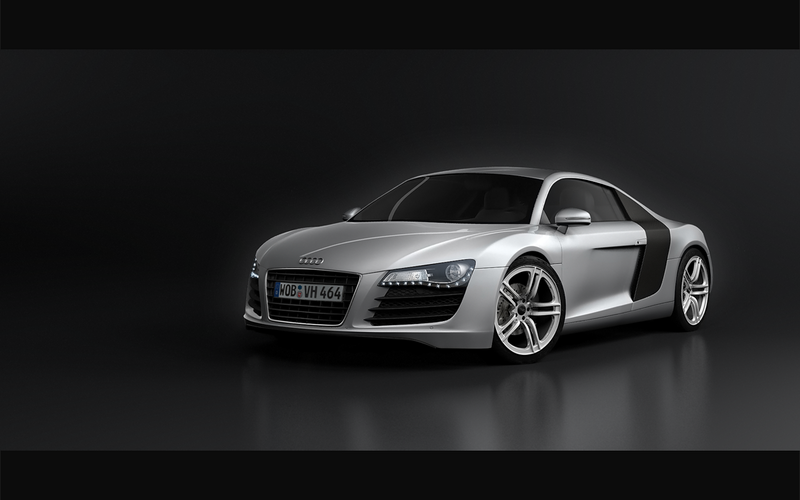
\includegraphics[scale=0.25]{audi.png}
\caption{Another R8 by Filip Sadlon}
\label{Another R8 by Filip Sadlon}
\end{center}
\end{minipage}
\hfill
\begin{minipage}[c]{.45\linewidth}
\begin{center}
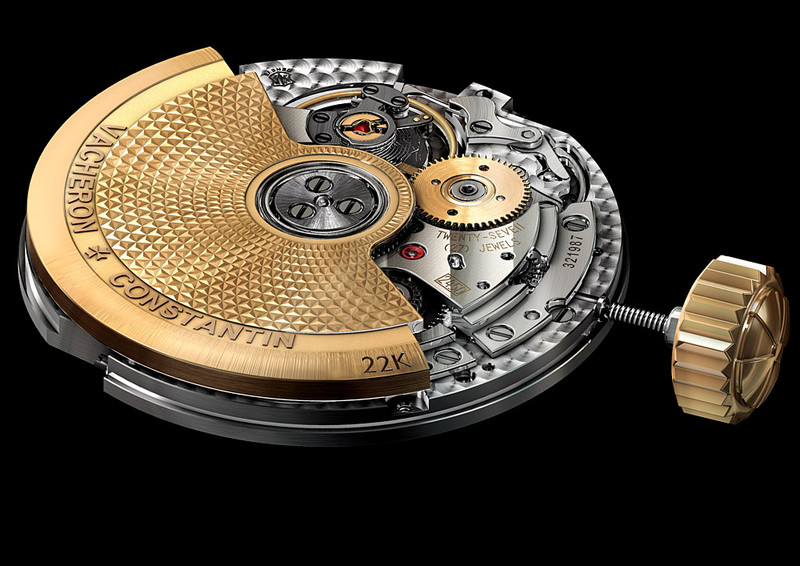
\includegraphics[scale=0.25]{watch.jpg}
\caption{3D Watch by Olivier Amrein}
\label{3D Watch by Olivier Amrein}
\end{center}
\end{minipage}
\end{figure}

\section{Installation}
Ich werde hier Ihnen die einfache Installation Blenders zeigen. Zuerst gehen Sie unter \url{http://www.blender.org/download/get-blender/} laden entweder die 64bits oder 32bits Version herunter. Sie m�ssen �berpr�fen ob sie einen x64 oder x86 Computer haben. Rechtklick auf "`Arbeitsplatz"', "`Eigenschaften"' 
und unter dem "`Allgemein"' Tab m�sste unter "`System"' entweder Microsoft Windows <Version> x64 Edition dann m�ssen Sie die 64bits Version Blenders herunterladen oder es steht nur einfach Microsoft Windows <Version> (<Version> gilt f�r die differenten Versionen Windows). Einmal das Sie Blender heruntergeladen haben f�hren Sie die Datei aus. Dann kommt ein erstes Men�: dr�cken Sie auf "`Next"' dann auf "`I Agree"', wieder auf "`Next"' und schliesslich auf "`Install"'. So, jetzt sollten Sie auf dem Desktop eine Icon die Blender heisst haben. Hier noch eine bildnerische Anleitung:

\bfseries Pr�fung der 32bits oder 64bits Version:
\begin{figure}[H]
\begin{center}
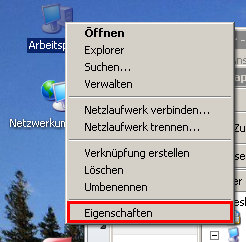
\includegraphics[scale=0.65]{Abb3_1_1.png}
\caption{Rechtklick auf "`Arbeitsplatz"', "`Eigenschaften"'}
\label{Rechtklick auf "`Arbeitsplatz"', "`Eigenschaften"'}
\end{center}
\end{figure}
\begin{figure}[H]
\begin{center}
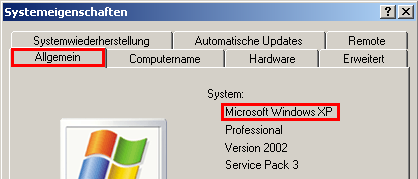
\includegraphics[scale=0.65]{Abb3_1_2.png}
\caption{"`Allgemein"' Tab}
\label{"`Allgemein"' Tab}
\end{center}
\end{figure}

\bfseries Installation Blenders:
\begin{figure}[H]
\begin{center}

\includegraphics[scale=0.65]{Abb3_1_3.png}
\caption{Doppelklick auf die heruntergeladene Datei}
\label{Doppelklick auf die heruntergeladene Datei}
\end{center}
\end{figure}

\begin{figure}[H]
\begin{center}
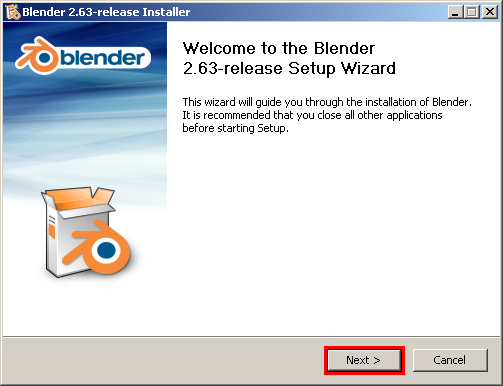
\includegraphics[scale=0.65]{Abb3_1_4.png}
\caption{"`Next"'}
\label{"`Next"'}
\end{center}
\end{figure}
\begin{figure}[H]
\begin{center}
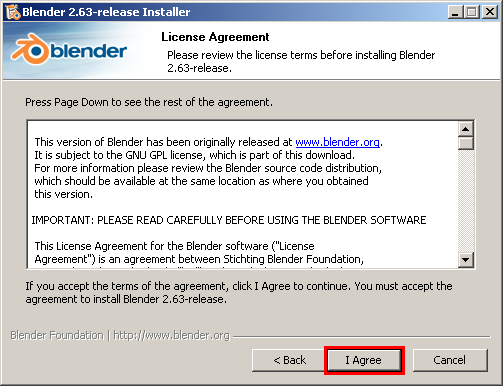
\includegraphics[scale=0.65]{Abb3_1_5.png}
\caption{"`I Agree"'}
\label{"`I Agree"'}
\end{center}
\end{figure}

\begin{figure}[H]
\begin{center}
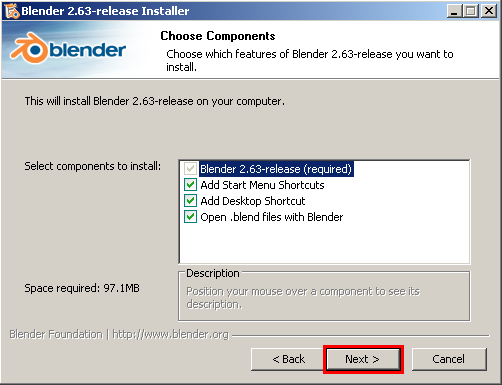
\includegraphics[scale=0.65]{Abb3_1_6.png}
\caption{"`Next"'}
\label{"`Next"'}
\end{center}
\end{figure}

\begin{figure}[H]
\begin{center}
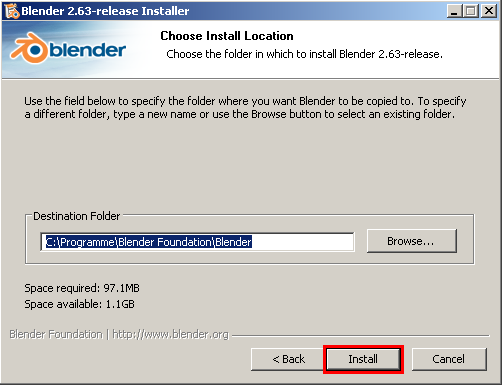
\includegraphics[scale=0.65]{Abb3_1_7.png}
\caption{"`Install"'}
\label{"`Install"'}
\end{center}
\end{figure}

\section{Mainmenu}
Doppelkicken Sie auf die "`Blender"' Icon somit er�ffnet es das Programm. Sie sollten dann auf einer solcher Oberfl�che gelangen.
\section{Objekte, meshs und co}
\section{Animationen}
\chapter{Textures}
\section{Zeichnen mit einer Tablet}
\section{Gimp}
\section{Photoshop}
\chapter{Website}
\section{Joomla Installation}
\section{Modifizierung des Layout}

\backmatter

\chapter{Nachwort}
\chapter{Quellen}
\bfseries Aus dem Internet:
\newline
Abb ~\ref{Blender Logo}: \url{http://download.blender.org/institute/logos/blenderlogo.png}
\newline Abb ~\ref{Another R8 by Filip Sadlon}: \url{http://www.blender.org/typo3temp/pics/7052dc1cb7.jpg}
\newline Abb ~\ref{3D Watch by Olivier Amrein}: \url{http://www.blender.org/typo3temp/pics/287897db88.jpg}
\end{document}
